%!TEX program = xelatex
\documentclass[color=green,mathpazo,titlestyle=hang,11pt]{elegantbook}

\author{Yu Wang}
\email{wyu0725@mail.ustc.edu.cn}
\zhtitle{FPGA}
\zhend{笔记}
\entitle{FPGA}
\enend{Note}
\version{1.0}
\myquote{吾生也有涯,而知也无涯.以有涯随无涯,殆已!已而为知者,殆而已矣!}
\logo{FPGAlogo.pdf}
\cover{FPGACover.pdf}

%green color
   \definecolor{main1}{RGB}{0,120,2}
   \definecolor{seco1}{RGB}{230,90,7}
   \definecolor{thid1}{RGB}{0,160,152}
%cyan color
   \definecolor{main2}{RGB}{0,175,152}
   \definecolor{seco2}{RGB}{239,126,30}
   \definecolor{thid2}{RGB}{120,8,13}
%blue color
   \definecolor{main3}{RGB}{20,50,104}
   \definecolor{seco3}{RGB}{180,50,131}
   \definecolor{thid3}{RGB}{7,127,128}

\usepackage{makecell}
\usepackage{lipsum}
\usepackage{texnames}
\usepackage{listings}
\usepackage{subfig}


\begin{document}
\maketitle
\tableofcontents
\mainmatter
\chapter*{说明}
最近看到两篇有意思的Xilinx White Paper,意识到也该把平时遇到的有意思的设计方面的内容记录下来,内容会慢慢的扩充.\\
本文档使用的模板来自于ElegantBook,网址已经停止维护了,但是其中一个作者的博客还在更新\href{http://ddswhu.com/}{Ethlisan},感谢作者提供模板
\part{FPGA介绍}

\part{Xilinx White Paper}
Xilinx公司有一系列的White Paper,口气不小,不过Xilinx工程师确实是有这个实力,写White Paper的工程师定是扫地僧式的人物。
\chapter{WP 275: Get your Priorities Right - Make your Design Up to 50\% Smaller}
\href{https://www.xilinx.com/support/documentation/white_papers/wp275.pdf}{文档下载地址},一开始学Verilog的时候把Verilog当成C一样的语言来学习,逐步了解到代码的背后是有硬件结构支持,也不是所有的代码都是可综合的,这一点暂时不讨论。这篇文档刷新了认识,代码背后不仅由硬件结构,还有基本的FPGA单元.这篇文档从LUT和D触发器入手介绍编译器是如何处理代码的。
\section{基本的逻辑实现}
\subsection{Single Level Logic}
首先考虑一个4输入与门的实现,代码如下\\
{\color{thid2}Verilog}
\begin{lstlisting}[language = Verilog, numbers=left,   
        numberstyle=\tiny,keywordstyle=\color{blue!70},  
        commentstyle=\color{red!50!green!50!blue!50},frame=shadowbox,  
        rulesepcolor=\color{red!20!green!20!blue!20},basicstyle=\ttfamily]  
always @(posedge clk) begin
  data_out <= a & b & c & d;
end
\end{lstlisting}  
{\color{thid2}VHDL}
\begin{lstlisting}[language = VHDL, numbers=left,   
        numberstyle=\tiny,keywordstyle=\color{blue!70},  
        commentstyle=\color{red!50!green!50!blue!50},frame=shadowbox,  
        rulesepcolor=\color{red!20!green!20!blue!20},basicstyle=\ttfamily]  
process (clk)
begin
	if clk’event and clk=’1’ then
		data_out <= a and b and c and d;
	end if; 
end process
\end{lstlisting} 
其实现如图\ref{Fig:SingleLevelLogic}所示,使用最简单的一个D触发器和一个4输入LUT即可实现
\begin{figure}[htbp]
	\centering
	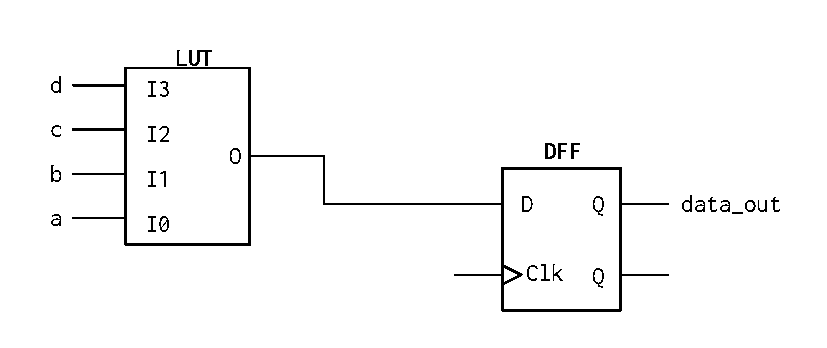
\includegraphics[width=0.7\textwidth]{figure/SingleLevelLogic.pdf}
	\caption{Single level logic use 4 input LUT and D Flip-Flop}
	\label{Fig:SingleLevelLogic}
\end{figure}
\subsection{Two Level Logic}
当逻辑门的输入个数增加之后,比如说增加到6个之后,LUT输入的个数显然不够了,这个时候就要使用两个LUT,如下图\ref{Fig:TwoLevelLogic}所示,这种情况无论如何2个LUT是免不了的。
\begin{figure}[htbp]
	\centering
	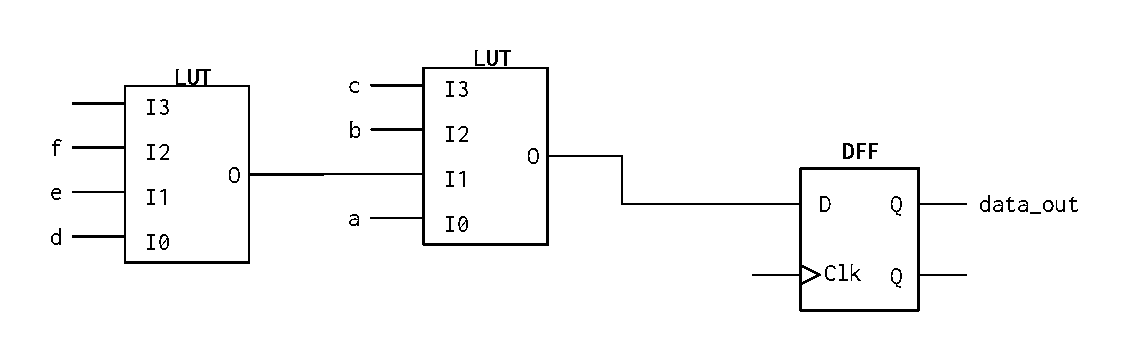
\includegraphics[width=0.7\textwidth]{figure/TwoLevelLogic.pdf}
	\caption{Two Level Logic use two 4-input LUT and a D Flip-Flop}
	\label{Fig:TwoLevelLogic}
\end{figure}
\section{D触发器中的同步和异步}
\subsection{添加Reset功能}
首先先在如下的VHDL代码中添加异步复位的功能
异步复位代码
%由于FPGA中的D触发器带有移步部分功能,实现如下\ref所示,这个例子似乎没有什么毛病
\subsection{添加更多的控制功能}
再看下一个例子,添加Reset和Enable的功能,如下代码所示
Enable和Reset功能的代码。
%这个时候Xilinx编译工具编译出来的结果就不是这么理想了,竟然用了两个4输入的LUT(\ref)
图
\{D触发器中的同步和异步不可得兼}
下面对这种情况进行解释,首先请回忆D触发器的类型,分为同步和异步两种D触发器,如下图\ref所示
\begin{figure}[htbp]
	\centering
	\subfloat[Synchronous DFF]{
	\label{fig:SynchromousDFF}
	\includegraphics{left.pdf}
	}
	\hspace{10pt}%
	\subfloat[Asynchronous DFF]{
	\label{fig:Asynchronous}
	\includegraphics{right.pdf}
	}
	\caption{Two different types DFF}
	\label{fig:TwoDFF}
\end{figure}
编译器必须要做出一个选择——使用同步的D触发器还是异步的D触发器,通常异步的D触发器优先级更高,因此会优先使用异步的D触发器,那么在有异步复位和同步置位的逻辑中,不可不免的会使用更多的D触发器来实现同步置位功能。\\
除此之外,使用两个Reset信号,一个是同步复位一个是异步复位也会出现这样的问题,可能你会感到奇怪,平时怎么会用到两个复位信号呢,还一个同步一个异步。其实不然,比如说下一个十进制计数器,计数器计到9之后会回到0,在编译器看来这就是复位,实际上代码中也会这么写,这无形中增加的同步复位会使得代码的资源量大大增加。\\
根据手册的说明,FPGA在上电配置完成之后会处在一个确定的状态,因此复位信号不一定是必须的,如果一定有必要设置一个复位信号,考虑同步的复位信号
\section{D触发器的优先级问题}
\subsectin{使用同步D触发器来实现代码}
说了不可以将同步和异步混着用,那么就是用同步复位、置位来实现代码,如下代码所示
不幸的是,编译器依旧将代码编译为两个LUT来实现(\ref),
\end{document}
